\documentclass[12pt]{article}

\usepackage{alphabeta}
\usepackage[greek, english]{babel}
\usepackage[utf8]{inputenc}
\usepackage{geometry}
\usepackage{graphicx}
\usepackage{amsmath}
\usepackage{float}

\graphicspath{{images/}}
\geometry{left=.3in, right=.3in, top=0.6in, bottom=0.6in}
\renewcommand{\baselinestretch}{1.2}
\pagenumbering{gobble}
\let\endtitlepage\relax

\begin{document}
%% ------ Title
    \begin{titlepage}
    \vspace*{-0.6in}
    \begin{flushleft}
        
\includegraphics[scale=0.44]{images/logo.png}
        
        \vspace{1cm}
        \textbf{Ονοματεπώνυμο:} Ανδρέας Γουλέτας (3170031), Λούντζης Λάμπρος (3170095)\\ 
        \textbf{Εργασία:} Τεχνητή Νοημοσύνη\\
        \textbf{Ημερομηνία:} 7 Δεκεμβρίου 2020
        
    \end{flushleft}
    \vspace{0.2in}
\end{titlepage}
%% -------------------------------------------------------------------------------------
\section*{Εισαγωγή}
Στο πρόβλημα \textbf{Bridge Crossing}, δοθέντος ενός συνόλου ατόμων, των χρόνων τους και μιας λάμπας, μας ζητείται να βρούμε την καλύτερη δυνατή διάσχηση των ατόμων από την μια πλευρά της γέφυρας στην άλλη. Οι περιορισμοί που τίθενται είναι οι εξής:
\begin{itemize}
    \item μπορούν να διασχύζουν την γέφυρα ζευγάρια των δύο ατόμων κάθε φορά (ένας θα κρατάει την λάμπα), και ο χρόνος που λαμβάνεται υπόψη είναι αυτός του αργότερου,
    \item πρέπει να γυρίζει ένα άτομο με την λάμπα πίσω κάθε φορά.
\end{itemize}
Για την λύση του προβλήματος αυτού κάνουμε χρήση του αλγορίθμου \textbf{A*}. Eπίσης, θα παρουσίασουμε μια σύγκρισή των αποτελεσμάτων που παράγει με αυτά του αλγορίθμου \textbf{BestFS}.
%% -------------------------------------------------------------------------------------
\section*{Dataset}
Για την αναπαράσταση των δεδομένων μας έχουμε επιλέξει αρχεία \textbf{CSV (Comma Separated Values)}. Η πρώτη γραμμή του αρχείου χρησιμοποιείται ως κεφαλίδα και αναφέρει ότι στην πρώτη στήλη θα πρέπει να υπάρχουν τα ονόματα των ατόμων (αλφαριθμητικά) ενώ στην δεύτερη στήλη οι χρόνοι τους (ακέραιοι αριθμοί μεγαλύτεροι του μηδενός).\\
Ενδεικτικό παράδειγμα αποτελεί το dataset1.csv στον φάκελο dataset. Τα άτομα και οι χρόνοι που περιέχονται είναι οι εξής:
\begin{itemize}
    \item George - 1 sec
    \item Nick - 3 sec
    \item Maria - 6 sec
    \item Kostas - 8 sec
    \item Lampros - 12 sec
\end{itemize}
%% -------------------------------------------------------------------------------------
\section*{Αλγόριθμος A*}
Για την εύρεση τελικής κατάστασης, δηλαδή μιας κατάστασης όπου όλα τα άτομα έχουν περάσει στην απέναντι πλεύρα της γέφυρας ή ο χρόνος έχει φτάσει ή υπερβεί το limitation, χρησιμοποιείται ο αλγόριθμος αναζήτησης A*.\\
Ο αλγόριθμος Α* χρησιμοποιεί πληροφόρηση και είναι \textbf{βέτιστος} και \textbf{πλήρης}. Για την αξιολόγηση των καταστάσεων χρησιμοποιείται η συνάρτηση
 \begin{equation*}
        f(n) = h(n) + g(n)
\end{equation*}\\
όπου n είναι ο κόμβος προς εξέταση, h είναι η ευρετική συνάρτηση που χρησιμοποείται και g είναι το κόστος της μετάβασης απο την κατάσταση-ρίζα στον κόμβο προς εξέταση.\\\\
\textbf{\underline{Παράδειγμα:}} Για είσοδο το παραπάνω dataset (dataset1.csv) και limit ίσο με 30sec, ο χρόνος που χρειάζονται τα άτομα να περάσουν στην απέναντι όχθη είναι 29sec.
%% -------------------------------------------------------------------------------------
\section*{Ευρετική Συνάρτηση}
Η ευρετική συνάρτηση που υλοποιήσαμε επιστρέφει ως αποτέλεσμα για κάθε κατάσταση το μέγιστο χρόνο από όλα τα άτομα που βρίσκονται στην όχθη εκκίνησης και δεν έχουν περάσει ακόμα.\\
Είναι αποδεκτή διότι αποτελεί υποεκτίμηση της πραγματικότητας, αφού αναιρεί και τους δυο περιορισμόυ που έχουν τεθεί (δυο άτομα διασχίζουν την γέφυρα κάθε φορά και ένα άτομα γυρνάει πίσω).
%% -------------------------------------------------------------------------------------
\section*{Σύγκριση με αλγόριθμο BestFS}
Ο αλγόριθμος BestFS σε αντίθεση με τον A* δεν χρησιμοποιεί πληροφόρηση, αλλά ούτε είναι πλήρης και βέλτιστος.  Για την αξιολόγηση των καταστάσεων χρησιμοποιείται η συνάρτηση
 \begin{equation*}
        f(n) = h(n)
\end{equation*}\\
όπου n είναι ο κόμβος προς εξέταση και h είναι η ευρετική συνάρτηση που χρησιμοποείται.\\\\
\textbf{\underline{Παράδειγμα:}} Για είσοδο το παραπάνω dataset (dataset1.csv) και limit ίσο με 30sec, ο χρόνος που χρειάζονται τα άτομα να περάσουν στην απέναντι όχθη είναι 46sec.\\\\
Για την σύγκριση των δύο αλγορίθμων χρησιμοποιήσαμε ώς είσοδο στο πρόγραμμα μας τέσσερα datasets (συμπεριλαμβανομένου και του παραπάνω παραδείγματος) χωρίς κάποιο limitation. Επίσης, χρησιμοποιείται η ίδια ευρετική συνάρτηση και στις δύο περιπτώσεις.\\
Από την γραφική παράσταση που ακολουθεί παρατηρούμε η έλλειψη πληροφόρισης έχει ως αποτέλεσμα να μην δίνεται η βέλτιστη δυνατή λύση, καθώς ο αλγόριθμος BestFS επιστρέφει λύσεις με μεγαλύτερο χρόνο διάσχησης συγκριτικά με τον αλγόριθμος Α*.
\begin{figure}[H]
        \centering
        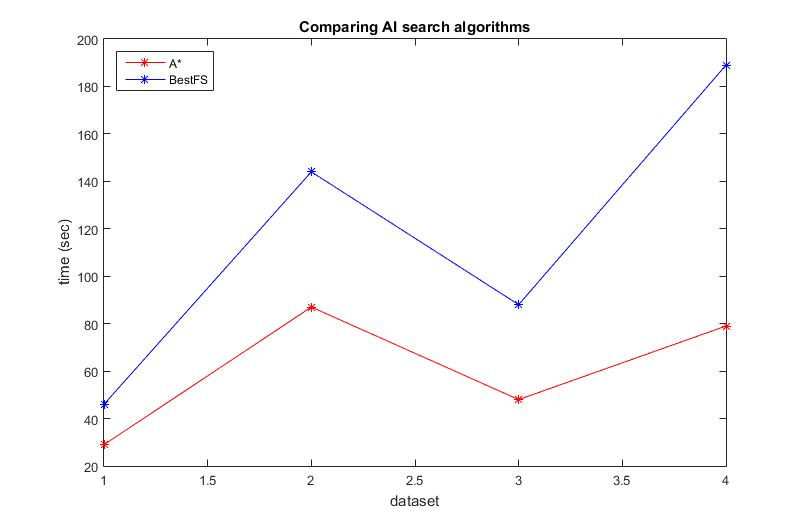
\includegraphics[scale=.7]{images/ai_res}
     \end{figure}
\end{document}
